\begin{figure}[H]
    \centering
    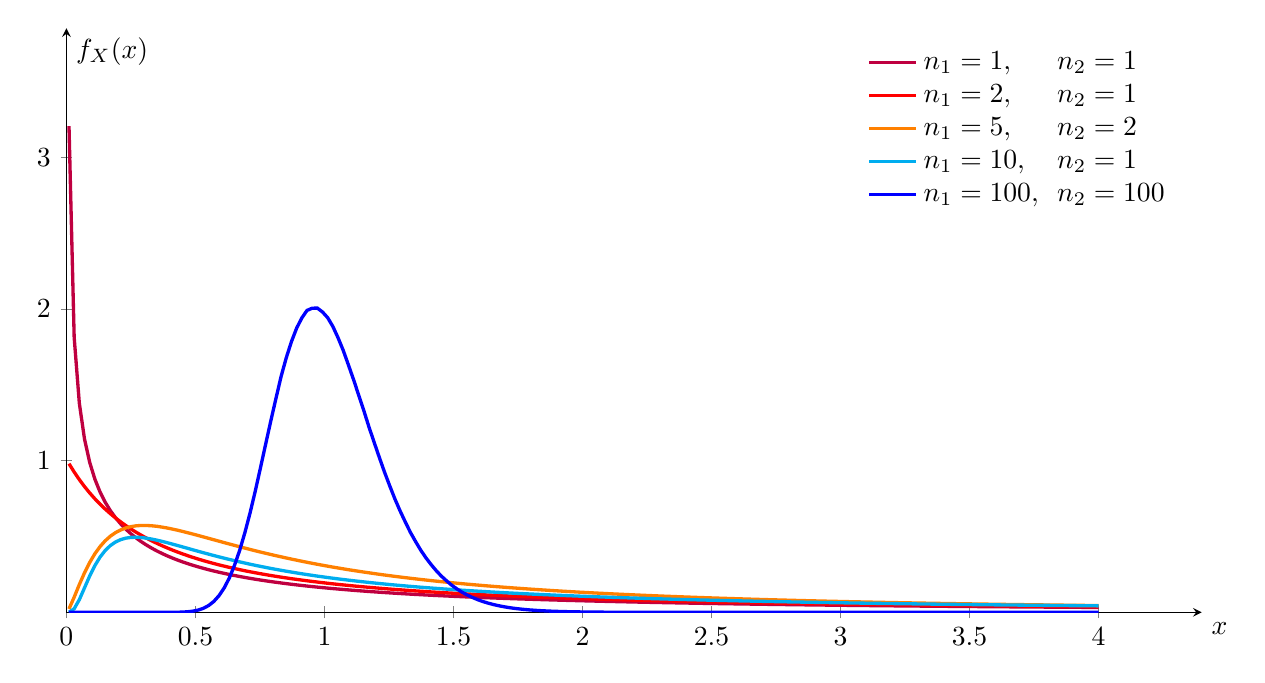
\begin{tikzpicture}[
        declare function={gamma(\z)=2.506628274631*sqrt(1/\z)+ 0.20888568*(1/\z)^(1.5)+ 0.00870357*(1/\z)^(2.5)- (174.2106599*(1/\z)^(3.5))/25920- (715.6423511*(1/\z)^(4.5))/1244160)*exp((-ln(1/\z)-1)*\z;},
        declare function={beta(\x,\y)=gamma(\x)*gamma(\y)/gamma(\x+\y);},
        declare function={fdst(\x,\a,\b) = 1 / beta(\a/2, \b/2) * (\a/\b)^(\a/2) * \x^(\a/2-1) * (1 + \a/\b*\x)^(-(\a + \b)/2);}
    ]
        \begin{axis}[
            axis lines = left,
            enlargelimits = upper,
            samples = 200,
            xmin = 0,
            ymin = 0,
            ymax = 3.5,
            ytick = {1, 2, 3},
            yticklabels = {1, 2, 3},
            xlabel = $x$,
            ylabel = $f_X(x)$,
            xlabel style = {at={(axis description cs:1,0)},anchor=north west},
            ylabel style = {at={(axis description cs:0,0.92)},anchor=south west,rotate=-90},
            domain=0.01:4,
            height = 9cm,
            width = 16cm,
            legend cell align = left,
            legend style = {draw=none}
        ]
            \addplot [very thick,purple] {fdst(x,1,1)}; \addlegendentry{$n_1=1,\hphantom{000} n_2=1$}
            \addplot [very thick,red] {fdst(x,2,1)}; \addlegendentry{$n_1=2,\hphantom{000} n_2=1$}
            \addplot [very thick,orange] {fdst(x,5,2)}; \addlegendentry{$n_1=5,\hphantom{000} n_2=2$}
            \addplot [very thick,cyan] {fdst(x,10,1)}; \addlegendentry{$n_1=10,\hphantom{00} n_2=1$}
            \addplot [very thick,blue] {fdst(x,100,100)}; \addlegendentry{$n_1=100,\hphantom{0} n_2=100$}
        \end{axis}
    \end{tikzpicture}
\end{figure}